% Created On: 2010.07.15
% Modified On: 2012.03.22
% Description: Ported MS thesis to PhD thesis .tex
% Modified On: 2014.03.26
% Description: Reformatted Document into form of actual dissertation. 
% Modified On: 2016.08.23 - Turned into a template file.
% Builds in WinEdt6.0 with Textify, then DVI-PDF. 
%%%%%%%%%%%%%%%%%%%%%%% preamble %%%%%%%%%%%%%%%%%%%%%%%%%%%
\documentclass[10pt,hyperref,normalmargins]{ucdthesis}
\usepackage{amssymb, amsmath, graphicx, subfigure, color, fancybox}
\usepackage{epstopdf}
\usepackage[utf8]{inputenc}
\usepackage[T1]{fontenc}
\usepackage{textcomp}
\usepackage{longtable}
\usepackage{float}
\usepackage{wrapfig}
\usepackage{soul}
\usepackage{amssymb}

\usepackage{url}  % helps hyperlinks
% Configure the linking of references and citations
\usepackage[dvipdfm, colorlinks=true, linkcolor=red, citecolor=blue, urlcolor=blue, linktoc=page]{hyperref}
\usepackage{cite}   % for Bibtex - needs to be after hyperref

\bibfiles{thesis_bib}

\title{Thesis Title}
\author{Thesis Writer}
\authorlastname{Thesis Writer Last Name}
\authorfirstname{Thesis Writer Firs Name + Middle Initial}
\bsdegree{B.S., Good University, City, State 2007}
\msdegree{M.S., Second University, City, State, 2011}

\setappendixtocdepth{3}

\principaladvisor{Joe Smith}
\principaladvisortitle{Associate Professor}
\committeechair{John Smith}
\firstreader{Katie Smith}
\secondreader{George Washington}
\thirdreader{Thomas Jefferson}
\departmenthead{Thomas Jefferson}
\department{Department of Biongineering}
\degree{Doctor of Philosophy}
\degreename{Ph.D. Bioengineering}
% Configuration parameters
\thesisproposaltrue    % flag to change from thesis to dissertation=true
\copyrightpagefalse     % optional
\contentspagetrue \figurespagefalse \tablespagefalse \bibpagetrue
\titlepagetrue
\dedicationheadingfalse
\multivolumefalse
\signaturepagetrue
\submitdate{2014} \numberwithin{equation}{chapter} \numberwithin{figure}{chapter}
\date{July 4, 1776}


%%%%%%%%%%%%%%%%%%%%%%% title page information %%%%%%%%%%%


 %\usepackage{ae} %%for Computer Modern fonts

\newcommand{\EQN}[0]{Eq. }
\newcommand{\FIG}[0]{Fig. }
\newcommand{\SEC}[0]{Sec. }
\newcommand{\CH}[0]{Ch. }
\newcommand{\TAB}[0]{Table }
\newcommand{\APX}[0]{Appendix }
\newcommand{\FDSDI}[0]{SPIFI }
\newcommand{\SPIFI}[0]{SPIFI }
\newcommand{\note}[1]{{\bf[#1]}}
\newcommand{\NA}[0]{$\rm{NA}$ }

% make subscripts roman


%%%%%%%%%%%%%%%%%%%%%%% begin %%%%%%%%%%%%%%%%%%%%%%%%%%%%%%
\begin{document}
\bibliographystyle{IEEEtran}

\begin{preliminary}
    \begin{abstract}
        Your abstract. 
    \end{abstract}

    \contents
%
%%    \begin{acknowledgements}
% %       To all the wonderful people in our group and that we collaborate with.
%%    \end{acknowledgements}
\end{preliminary}

%%%%%%%%%%%%%%%%%% title page information %%%%%%%%%%%%%%%%%%


%\end{thebibliography}      % From template

%%%%%%%%%%%%%%%%%%%%%%%%%%  body  %%%%%%%%%%%%%%%%%%%%%%%%%%
\chapter{Introduction}
My Introducdtion.

\section{Specific Aims}

\section{Background \& Significance}


\section{Innovation}

\chapter{Sub Project 1}
Chapter structures are pretty flexible. Some may prefer a Introduction, Methods, Results, Discussion approach. Take an approach that describes the project with the most clarity. 

 ere is an example of how to insert a figure. Size the eps files for input so it doesn't have to be scaled. Scaling can be added using the includegraphics[] tag. 
\begin{figure}[h]
    \begin{centering}
    \subfigure[Phase Distribution of Perfect Lens and Phase Accumulated to the lens plane]{
    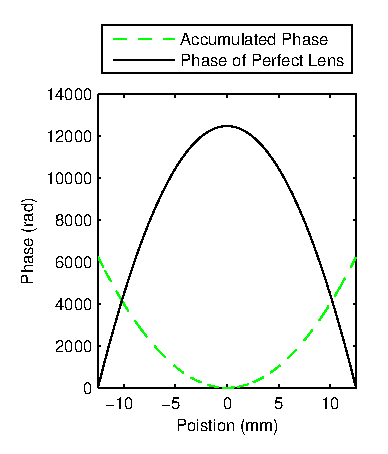
\includegraphics[]{Graphics/Point_Spread_Function/perfect_lens_phase.eps}
    % Generated from \Software\MATLAB\Spiffi\psfSingleLens_mag1.m
    \label{fig: phase perfect lens}}
    \subfigure[Point Spread Functions]{
    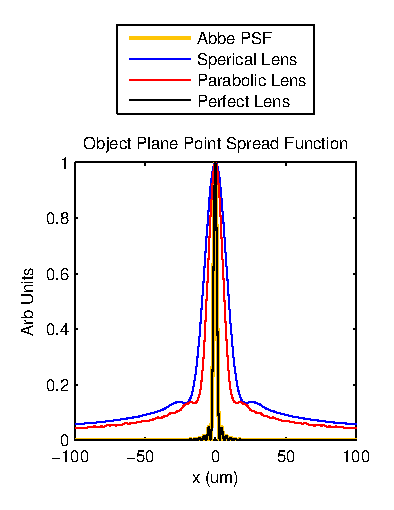
\includegraphics[]{Graphics/Point_Spread_Function/psf_perfect_lens.eps}
    % Generated from \Software\MATLAB\Spiffi\psfSingleLens_mag1.m
    \label{fig: PSF Perfect Lens}}
    \caption[]{Phase Distribution for a perfect lens \subref{fig: phase perfect lens}. The accumulated phase(green) is in the apostate direction of the perfect lens(black).  \subref{fig: PSF Perfect Lens} shows a comparison of PSFs of the perfect lens(black) to the previous ones of the spherical lens(blue) and parabolic lens(red). The PSF of the prefect lens overlaps Abbe PSF(gold).
    \label{fig: Perfect Lens}}
    \end{centering}
\end{figure}

Now you can reference \ref{fig: PSF Perfect Lens} in your text. 

You can reference someoneelses work like this. The Abbe diffraction limit was first published \cite{abbe_relation_1882} . 

\chapter{Sub Project 2}

\chapter{Sub Project 3}

\chapter{Evaluation of Biomarker Panel in CTCs Isolated from Ovarian and Prostate Cancer Patients}


\begin{postliminary}

%\references
% Needed for winedt to see citations

% this can be generated in a tool such as zotero. Encourage using UTF-8 encoding
\bibliography{thesis_bib}

\end{postliminary}


\end{document}
